%!TEX root =  main.tex
\section{Introduction}

Designing scalable and highly available services is the holy grail of many distributed systems designers.
%Many online services have demanding performance and availability requirements.
%To implement scalable and highly available services system designers typically recur to state partitioning and replication.
Two of the most important techniques used to achieve scalability and high availability are state partitioning and replication.
By partitioning the service state (i.e., sharding), each partition can contribute to overall performance.
In principle, performance should increase with the number of partitions.
By replicating state in multiple servers, the system can be configured to tolerate any number of server failures.

Although there are numerous accounts of distributed systems that rely on state partitioning and replication (e.g., \cite{x,y,z,w}), descriptions of how to partition the state of a service are less common (e.g., \cite{curino2010sch}).
%most papers assume that partitioning is provided by the application designer or system operator.
This paper considers the problem of state partition in the context of Scalable State Machine Replication (S-SMR) [8], a technique that partitions the service state and replicates each partition.
Even though the discussion is centered on S-SMR, it is relevant to other techniques that partition the state and guarantee strong consistency (e.g., \cite{xxx}).
%
%Replication and partitioning introduce tradeoffs, the most emblematic of which being the consistency of the service.
%\emph{Weakly consistent} services expose to the clients the existence of replicas and partitions.
%For example, clients may not see state changes performed by previously completed operations since these may have been applied to some replicas, but not ``enough replicas". 
%\emph{Strongly consistent} services strive to hide replication and partitioning from clients.
%In this case, the service behaves to the clients as if it was implemented by a single server.
%While weakly consistent services can be more efficiently implemented than strongly consistent services and are less exposed to impossibility results~\cite{FLP85,Gilbert:2002},
%they may offer non-intuitive behavior to clients.
%
%Due to the importance of providing services that clients can intuitively understand, several approaches have been proposed that do not sacrifice consistency (e.g., [11, 21, 30, 31]).
%This paper focuses on Scalable State Machine Replication (S-SMR) [8], a technique that partitions the service state and replicates each partition.
%Our argument, however, holds for other solutions that partition the state and guarantee strong consistency.
S-SMR relies on an atomic multicast primitive to consistently order commands within and across partitions. 
Commands that access objects located in a single partition (i.e., single-partition commands) are multicast to the concerned partition and executed like in classical SMR. 
Commands that access objects located in multiple partitions (i.e., multi-partition commands) are multicast to all involved partitions.
To prevent command interleaves that violate strong consistency, partitions coordinate during the execution of multi-partition commands.

Because single-partition commands are much more efficient than multi-partition commands (i.e., in some cases by a factor of more than 10x), the performance of S-SMR is particularly sensitive to the way the service state is partitioned.
But partitioning the service state with the goals of maximizing single-partition commands and minimizing load imbalances among partitions is challenging for at least two reasons.
First, a favorable partitioning requires detailed a priori information about the service workload (i.e., which commands access which objects).
Second, even if enough information is available, workloads change over time (e.g., in social networks users join and leave the system, connections are created and removed), which requires the partitioning to be revisited as the system evolves.

In light of these challenges, state partitioning needs to be \emph{dynamic} and adapt to workload changes on-the-fly, as opposed to \emph{static}, in which the partitioning is defined before the system starts and re-partitioning the state requires system shutdowns.
Long et al.~\cite{hoang2016} propose a dynamic partitioning scheme that turns every multi-partition command into a single-partition command by moving the objects needed by a command to a single partition before the command is executed.
%The scheme relies on clients to decide where to group objects and largely outperforms static schemes (e.g., \cite{bezerra2014ssmr}) in workloads that provide a high degree of locality.
In this scheme, which hereafter we refer to as \emph{decentralized partitioning}, clients decide to which partition the objects needed by a command should be moved.
In workloads that exhibit \emph{strong locality} (defined next), the decentralized scheme makes the system eventually converge to a partitioning in which no further moves are needed.
When this happens, performance scales with the number of partitions deployed.

We define locality using a \emph{workload graph} in which vertices are objects (the service state) and edges are commands. 
%To define locality, assume that the workload is represented by a graph in which vertices are objects, the service state, and edges interconnect objects accessed by a command. 
An edge between two objects models commands that access the two objects.
Strong locality means that the workload graph contains connected components.
Intuitively, the decentralized scheme works because eventually every connected component is entirely hosted by a partition, and once this happens no further object moves are needed to execute commands, that is, the system converges.
In the presence of \emph{weak locality}, however, the system never converges: objects permanently need to change partition, which hurts performance.

\begin{figure*}[ht]
	\center
	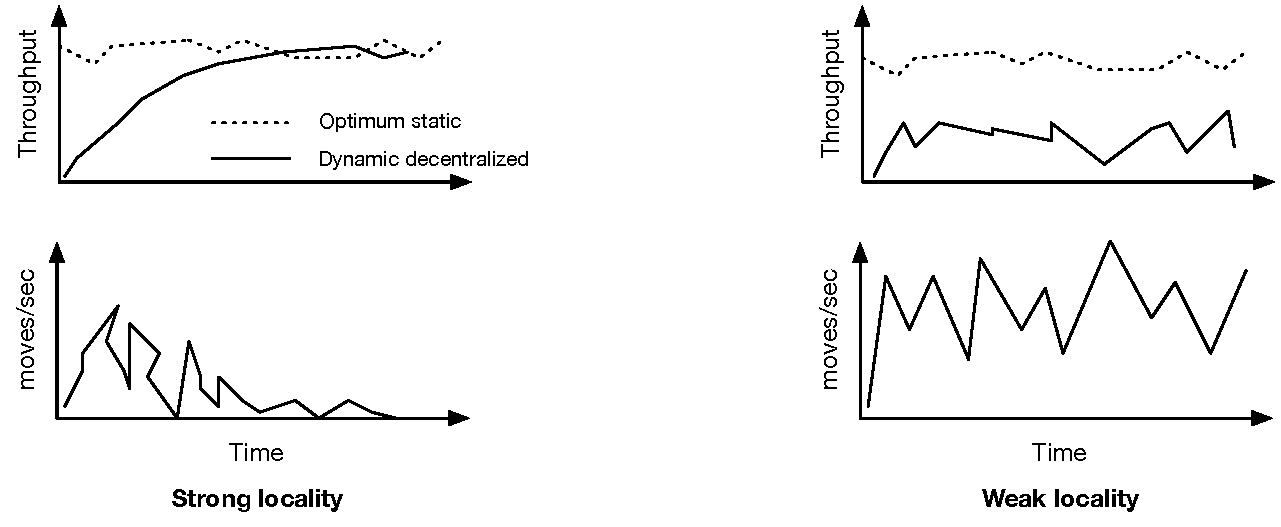
\includegraphics[width=0.6\linewidth]{figures/motivation}
	\caption{Performance under strong and weak locality.}
	\label{fig:motivation}
\end{figure*}

To illustrate our point, we experimentally evaluate the decentralized scheme proposed by Long et al.~\cite{hoang2016} with workloads that exhibit strong and weak locality.
We also compare the technique to an optimized static partitioning scheme, hereafter, referred to as \emph{optimized partitioning}.
The optimized partitioning scheme uses METIS~\cite{Abou-Rjeili:2006} to compute a partitioning of the workload graph and then distribute objects among partitions before the system starts.
METIS creates balanced partitions with a near-minimum number of edges across partitions.
In the decentralized partitioning scheme, objects are randomly distributed among partitions at startup and then moved across partitions as the execution evolves.
With strong locality, METIS decomposes the workload graph into connected components, one per partition.
With weak locality, METIS partitions the workload so that approximately 1\% of edges connect objects in different partitions.
Notice that the optimized scheme is intended as a reference for performance, as it requires complete a priori knowledge about the workload.

Figure~\ref{fig:motivation} shows the results.
With strong locality, the decentralized scheme experiences a large number of move operations until each connected component is entirely contained in a partition (left top graph).
Once this happens, throughput of the scheme is similar to the throughput of the optimized scheme (left bottom graph).
With weak locality, though, move operations happen throughout the whole execution (right top graph).
In this case, throughput is substantially lower than what the optimized scheme can achieve (right bottom graph).
%This essentially happens because move commands followed by a single-partition command are more expensive than a multi-partition command

In this paper, we introduce \dynastar, a dynamic partitioning scheme for state machine replication that is inspired by the optimized static scheme but does not require any a priori knowledge about the workload.
%\dynastar converges to the performance of the optimized static scheme by collecting workload information during the execution and periodically computing a partitioning of the service state using a graph partitioning algorithm (in our case METIS).
%
In its simplest form, \dynastar works as follows.
As in S-SMR, a location oracle keeps track of the partition where each object is stored.
In \dynastar, in addition to storing the mapping of objets to partitions, the oracle also builds a workload graph with objects as vertices and edges as commands that access the objects. 
To submit a command, clients consult the location oracle to find out the partition the command must be multicast to.
If the command accesses objects in multiple partitions, the oracle updates the workload graph with the command and moves objects to a single destination partition, after which the client can multicast the command.
In order to choose the ``right" destination partition for the objects of a command, the oracle periodically computes a partitioning of the workload graph with METIS and uses the resulting partitioning as a reference to decide where to move the objects to.
The oracle uses two heuristics to decide the destination partition of the objects of a command.
First, it tries to move the minimum number of objects.
Second, it attempts to respect as much as possible the partitioning of the workload graph.

We have fully implemented \dynastar and compared its performance to the dynamic partitioning protocol proposed by Long et al.~\cite{hoang2016} and to the optimized static partitioning scheme.
Our prototype can handle workload graphs with half a million objects and tens of millions of connections.
In workloads that present strong locality, all three protocols eventually delivered comparable performance, although \dynastar converged more quickly than the decentralized scheme.
In workloads with weak locality, however, \dynastar \emph{outperformed both} schemes.
The reason for the surprisingly high performance of \dynastar compared to the optimized static partitioning scheme is that \textbf{we need to explain this!!! :-)}

The paper makes the following contributions:
\begin{itemize}
\item It introduces \dynastar and discusses its implementation. 
\item It evaluates different partitioning schemes for state machine replication under a variety of conditions.
\item It describes \appname{} to demonstrate how \libname{} can be used to implement a scalable social network service.
\item It presents a detailed experimental evaluation of \dynastar including real social network graphs with half a million users and 14 million edges.
\end{itemize}

The rest of the paper is structured as follows.
Section~\ref{sec:sysmodel} describes our system model.
Section~\ref{sec:background} reviews existing scalable state machine replication approaches.
Section~\ref{sec:dssmr} introduces \dssmr{}; we explain the technique in detail and argue about its correctness.
Section~\ref{sec:implementation} details the implementation of \libname\ and \appname{}.
Section~\ref{sec:experiments} reports on the results of our experiments with \dssmr{}.
Section~\ref{sec:rw} surveys related work and
Section~\ref{sec:conclusion} concludes the paper.



%The main contribution of this paper is a dynamic partitioning scheme that \emph{performs comparably to the optimum static scheme but with no a priori knowledge about the workload}.


%%State machine replication (SMR) is a well-established technique to develop highly available services (e.g., \cite{Shvachko:2003,Ghemawat:2003,Burrows:2006,MacCormick:2004}).
%%In essence, the idea is that replicas deterministically execute the same sequence of client commands in the same order and in doing so traverse the same sequence of states and produce the same results.
%%State machine replication provides configurable fault tolerance in the sense that the system can be set to tolerate any number of faulty replicas.
%%%Increasing the number of replicas, however, will not scale performance since each replica must execute every command.
%%Unfortunately, increasing the number of replicas will not scale performance since each replica must execute every command.
%%
%%%For many online services, caping performance is a serious drawback.
%%Conceptually, scalable performance can be achieved with state partitioning (e.g., \cite{facebookTAO, sciascia2012sdur, Aguilera:2007}).
%%Ideally, if the service state can be divided such that commands access one partition only and are equally distributed among partitions, then system throughput (i.e., the number of commands that can be executed per time unit) will increase linearly with the number of partitions.
%%Although promising, exploiting partitioning in SMR is challenging.
%%First, most applications cannot be partitioned in such a way that commands always fall within a single partition.
%%Therefore, a partitioning scheme must cope with multi-partition commands.
%%Second, determining an efficient partitioning of the state is computationally expensive and requires an accurate characterization of the workload.
%%
%%There are two general solutions to handle multi-partition commands.
%%One solution is to weaken the guarantees of commands that involve multiple partitions (e.g., \cite{facebookTAO}).
%%In the context of SMR, this would mean that single-partition commands are strongly consistent (i.e., linearizable) but multi-partition commands are not.
%%Another solution is to provide strong consistency guarantees for both single- and multi-partition commands, at the cost of a more complex execution path for commands that involve multiple partitions.
%%\ssmrlong\ (\ssmr)~\cite{bezerra2014ssmr} is a solution in this category.
%%\ssmr\ partitions the service state and replicates each partition.
%%It relies on an atomic multicast primitive to consistently order commands within and across partitions. 
%%Single-partition commands are multicast to their concerned partition and executed just like in classical SMR.
%%Multi-partition commands are multicast to all involved partitions; to prevent command interleaves that violate strong consistency, \ssmr\ implements execution atomicity.
%%With execution atomicity, partitions coordinate during the execution of multi-partition commands.
%%Unsurprisingly, multi-partition commands are more expensive than single-partition commands, and thus, the performance of \ssmr\ is particularly sensitive to the way the service state is partitioned.
%%
%%Determining a partitioning of the state that avoids load imbalances and favors single-partition commands normally requires a good understanding about the workload. 
%%Even if enough information is available, finding a good partitioning is a complex optimization problem~\cite{curino2010sch,taft2014est}.
%%Moreover, many online applications experience variations in demand. 
%%These happen for a number of reasons. 
%%In social networks, some users may experience a surge increase in their number of followers (e.g., new ``celebrities");
%%workload demand may shift along the hours of the day and the days of the week; and unexpected (e.g., a video that goes viral) or planned events (e.g., a new company starts trading in the stock exchange) may lead to exceptional periods when requests increase significantly higher than in normal periods.
%%\ssmr\ assumes a static workload partitioning.
%%Any state reorganization requires system shutdown and manual intervention.
%%
%%Given these issues, it is crucial that highly available partitioned systems be able to dynamically adapt to the workload.
%%In this paper, we present \dssmrlong\ (\dssmr), a technique that allows a partitioned SMR system to reconfigure its data placement on-the-fly.
%%\dssmr\ achieves dynamic data reconfiguration without sacrificing scalability or violating the properties of classical SMR.
%%These requirements introduce significant challenges.
%%Since state variables may change location, clients must find the current location of variables.
%%The scalability requirement rules out the use of a centralized oracle that clients can consult to find out the partitions a command must be multicast to.
%%Even if clients can determine the current location of the variables needed to execute a command, by the time the command is delivered at the involved partitions one or more variables may have changed their location.
%%Although the client can retry the command with the new locations, how to guarantee that the command will succeed in the second attempt?
%%In classical SMR, every command invoked by a non-faulty client always succeeds.
%%\dssmr\ should provide similar guarantees.
%%
%%\dssmr\ was designed to exploit workload locality.
%%Our scheme benefits from simple manifestations of locality, such as commands that repeatedly access the same state variables, and more complex manifestations, such as structural locality in social network applications, where users with common interests have a higher probability of being interconnected in the social graph.
%%Focusing on locality allows us to adopt a simple but effective approach to state reconfiguration: whenever a command requires data from multiple partitions, the variables involved are moved to a single partition and the command is executed against this partition.
%%To reduce the chances of skewed load among partitions, the destination partition is chosen randomly.
%%Although \dssmr\ could use more sophisticated forms of partitioning, formulated as an optimization problem (e.g., \cite{curino2010sch,taft2014est}), our technique has the advantage that it does not need any prior information about the workload and is not computationally expensive.
%%
%%To track object locations without compromising scalability, in addition to a centralized oracle that contains accurate information about the location of state variables, each client caches previous consults to the oracle.
%%As a result, the oracle is only contacted the first time a client accesses a variable or after a variable changes its partition.
%%Under the assumption of locality, we expect that most queries to the oracle will be accurately resolved by the client's cache.
%%To ensure that commands always succeed, despite concurrent relocations, after attempting to execute a command a few times unsuccessfully, \dssmr\ retries the command using \ssmr{}'s execution atomicity and involving all partitions. 
%%Doing so increases the cost to execute the command but guarantees that relocations will not interfere with the execution of the command.
%%
%%We have fully implemented \dssmr\ as the \libname{} Java library, and we performed a number of experiments using \appname{}, a social network application built with \libname{}.
%%%, with workloads exhibiting weak and strong locality.
%%We compared the performance of \dssmr\ to \ssmr\ using different workloads.
%%With a mixed workload that combines various operations issued in a social network application, \dssmr\ reached 74~kcps (thousands of commands per second), against less than 33~kcps achieved by \ssmr{}, improving by a factor of over 2.2.
%%Moreover, \dssmr's performance scales with the number of partitions under all workloads.
%%%With a weak-locality workload, \dssmr\ reached XX~kcps, against YY~kcps of \ssmr{}.
%%
%%The paper makes the following contributions:
%%(1) It introduces \dssmr\ and discusses some performance optimizations, including the caching technique. 
%%(2) It details \libname{}, a Java library to simplify the design of services based on \dssmr{}.
%%(3) It describes \appname{} to demonstrate how \libname{} can be used to implement a scalable social network service.
%%(4) It presents a detailed experimental evaluation of \appname{}, deploying it with \ssmr\ and \dssmr{} in order to compare the performance of the two replication techniques.
%%
%%The rest of the paper is structured as follows.
%%Section~\ref{sec:sysmodel} describes our system model.
%%Section~\ref{sec:background} reviews SMR and \ssmrshort{}.
%%Section~\ref{sec:dssmr} introduces \dssmr{}; we explain the technique in detail and argue about its correctness.
%%Section~\ref{sec:implementation} details the implementation of \libname\ and \appname{}.
%%Section~\ref{sec:experiments} reports on the results of our experiments with \dssmr{}.
%%Section~\ref{sec:rw} surveys related work and
%%Section~\ref{sec:conclusion} concludes the paper.
%%
%%
